% Оформление по ГОСТ (Положение о ВКР МФТИ): шрифт Times New Roman 14 pt,
% межстрочный интервал 1,5, поля 30/15/20/20 мм, абзацный отступ 1,25 см,
% список литературы по ГОСТ Р 7.0.5-2008 (biblatex-gost).
\documentclass[14pt, a4paper]{extarticle}

\usepackage[a4paper, left=30mm, right=15mm, top=20mm, bottom=20mm]{geometry}
\usepackage[T2A]{fontenc}
\usepackage[utf8]{inputenc}
\usepackage[english, russian]{babel}
\usepackage{mathtools}        % подгружает amsmath
\usepackage{amsthm}
\usepackage{tempora}          % Times-подобный текстовый шрифт с кириллицей (T2A)
\usepackage{newtxmath}        % Times-подобная математика (после tempora)
\usepackage{booktabs}
\usepackage{array}
\usepackage{graphicx}
\graphicspath{{../figures/}{figures/}}
\usepackage{setspace}
\onehalfspacing               % межстрочный интервал 1,5
\setlength{\parindent}{1.25cm}
\usepackage[autostyle]{csquotes}
\usepackage[colorlinks=true, linkcolor=blue, citecolor=blue, urlcolor=blue]{hyperref}
\usepackage[backend=biber, style=gost-numeric, sorting=none, language=auto]{biblatex}
\addbibresource{references.bib}
\appto{\bibsetup}{\emergencystretch=1.5em}
\pagestyle{plain}             % номер страницы внизу по центру

\theoremstyle{definition}
\newtheorem{definition}{Определение}[section]
\newtheorem{remark}[definition]{Замечание}
\newtheorem{example}[definition]{Пример}
\newtheorem{assumption}[definition]{Предположение}

\theoremstyle{plain}
\newtheorem{theorem}[definition]{Теорема}
\newtheorem{proposition}[definition]{Утверждение}
\newtheorem{lemma}[definition]{Лемма}
\newtheorem{corollary}[definition]{Следствие}

\title{Геометрический подход к оценке сложности данных\\ на основе генеративных диффузионных моделей}
\author{Д.\,А.~Черноусов\\ \small Научный руководитель: А.\,В.~Грабовой, к.ф.-м.н.}
\date{\today}


\makeatletter
\renewenvironment{proof}[1][\proofname]{\par
    \pushQED{\qed}%
    \normalfont \topsep6\p@\@plus6\p@\relax
    \trivlist
    \item[\hskip\labelsep\itshape #1\@addpunct{.}]\mbox{}\\*
    \ignorespaces
}{\popQED\endtrivlist\@endpefalse}
\makeatother


\begin{document}

% ==========================================================================
% Титульный лист (оформление шаблона ВКР ФПМИ, как у Кравацкого)
% ==========================================================================
\thispagestyle{empty}
\begin{titlepage}
\begin{center}
Федеральное государственное автономное образовательное учреждение\\ высшего образования\\
<<Московский физико-технический институт\\
(национальный исследовательский университет)>>\\
Физтех-школа прикладной математики и информатики\\
Кафедра интеллектуальных систем
\end{center}

\vspace{0pt plus5fill}

\begin{center}
\large{Черноусов Данила Владиславович}
\end{center}

\vspace{0pt}

\begin{center}
\textbf{\large{\MakeUppercase{Геометрический подход к оценке сложности данных на основе генеративных диффузионных моделей}}}
\end{center}

\vspace{0pt}

\begin{center}
03.03.01~--- Прикладные математика и физика
\end{center}

\vspace{0pt}

\begin{center}
Выпускная квалификационная работа бакалавра
\end{center}

\vspace{0pt plus2fill}

\begin{center}
\hfill\parbox{8.4cm}{\textbf{Научный руководитель:}\\
Грабовой Андрей Валериевич,\\
кандидат физико-математических наук}\\
\vspace{0pt plus4fill}
Москва~--- 2026
\end{center}
\end{titlepage}
\setcounter{page}{2}

\newpage
\begingroup
\hypersetup{linkcolor=black}
\tableofcontents
\endgroup

\newpage
\begin{center}
    \Large\textbf{Аннотация}
\end{center}

\noindent
Во многих задачах машинного обучения важно оценивать не только объём, но и
разнообразие обучающей выборки, причём без опоры на разметку: это нужно для
прогнозирования качества моделей, для отбора обучающих подвыборок и для сравнения
наборов данных одного объёма, но разного содержания. Существующие меры сложности
данных описывают лишь локальную размерность или опираются на готовые признаковые
представления и не улавливают семантическую геометрию порождающего распределения,
то есть то, насколько объекты выборки близки по смыслу и на каких масштабах. В
работе предлагается извлекать эту геометрию из предобученной диффузионной модели:
каждому объекту сопоставляется его траектория в порождающем процессе, описывающая
объект сразу на всех масштабах, а сложность выборки оценивается как эффективный
объём, который она занимает в пространстве траекторий. Установлены достаточные
условия корректности меры и доказаны теоремы о её свойствах, предложен способ её
вычисления через траектории диффузионной модели,экспериментально показано семантическая согласованность предложенной меры.

\newpage
% ==========================================================================
\section{Введение}
\label{sec:intro}
% ==========================================================================

Качество модели машинного обучения определяется не только объёмом обучающей
выборки: две выборки одинакового размера могут заметно различаться по
разнообразию и информативности, а с ними и по тому, насколько сложную модель они
позволяют обучить и насколько хорошо она обобщает~\cite{Mei2022Towards,Konz2024Effect}.
Это видно уже на простых примерах. Набор из тысяч почти одинаковых кадров одного
видеоролика или из множества сдвигов и небольших поворотов одного изображения
формально велик, но содержательно беден: все его объекты получены из одного и
почти не добавляют разнообразия~\cite{Chen2020GroupAugmentation}. По той же
причине число токенов, привычная ось в законах масштабирования
качества~\cite{Kaplan2020ScalingLaws}, слабо отражает информативность текстового
корпуса: токены сильно зависимы и избыточны~\cite{Chen2025SubScaling}, и удаление
дубликатов или отбраковка лишних примеров способны не ухудшить обучение, а
улучшить его~\cite{Lee2022Deduplicating,Sorscher2022BeyondScaling}. В подобных
случаях информативен не объём, а эффективный размер выборки. Это понятие давно
формализовано в статистике: зависимые или избыточные наблюдения несут меньше
информации, чем столько же независимых, и реальное число объектов может
многократно превышать эффективный размер
выборки~\cite{Kish1965Survey,Geyer1992MCMC}. Поэтому возникает потребность в мере
сложности выборки, которая численно отражала бы это разнообразие и была бы
согласована с геометрией порождающего распределения. Такая мера полезна для
прогнозирования качества модели по характеристикам данных, для адаптивного
обучения, то есть отбора обучающих подвыборок с учётом их
сложности~\cite{Bengio2009Curriculum,Kumar2010SelfPaced}, и для сравнения наборов
данных одного объёма, но разного содержания~\cite{Swayamdipta2020Cartography,Rahane2020Measures}.

Существующие меры сложности данных можно разделить на два рода. Одни оценивают
сложность задачи классификации по размеченной выборке: меры перекрытия признаков
и разделимости классов Хо и Басу~\cite{Ho2002Complexity}, систематизированные в
обзоре~\cite{Lorena2019Complexity}, оценки трудности отдельных
объектов~\cite{Smith2014Instance}, а также классические меры ёмкости класса
гипотез, размерность Вапника--Червоненкиса~\cite{Vapnik1971Uniform} и сложность
Радемахера~\cite{KoltchinskiiPanchenko2000Rademacher}. Все они отвечают на вопрос,
насколько трудно выучить разметку, и не определены без меток.

Другие меры оперируют только объектами, без меток. Сюда относятся оценки
внутренней размерности многообразия данных, в том числе с помощью диффузионных
моделей~\cite{Tempczyk2022LIDL,Kamkari2024Geometric}, и информационные меры на
основе энтропии и взаимной информации~\cite{CoverThomas2006}. Ближайшее к
предлагаемой мере семейство, спектральные меры разнообразия, сводит выборку к
спектру положительно полуопределённой матрицы похожести:
Vendi Score~\cite{FriedmanDieng2023Vendi} и его обобщение на порядки
Реньи~\cite{PasarkarDieng2024Cousins} берут экспоненту энтропии нормированного
спектра, а лог-детерминантный объём детерминантных точечных
процессов~\cite{KuleszaTaskar2012DPP} и эффективный
ранг~\cite{RoyVetterli2007EffectiveRank} суть родственные спектральные функционалы
того же ядра. Примыкает направление оценки достаточного объёма выборки и
сложности моделей~\cite{Gadaev2022Sample,GrabovoyStrijov2022Distillation,Grabovoy2025Thesis}.

Общий недостаток перечисленных подходов в том, что они либо описывают лишь
локальную размерность, либо опираются на готовые признаковые представления и не
учитывают семантическую геометрию порождающего распределения: то, насколько
объекты выборки близки или далеки по смыслу и на каких масштабах.

В настоящей работе семантическая геометрия данных извлекается из предобученной
диффузионной модели. Такая модель кодирует геометрию многообразия данных: по её
скор-функции строятся римановы метрики на пространстве
данных~\cite{Azeglio2025Inside}, а её детерминированные траектории несут
содержательную семантическую информацию об объекте. Детерминированная траектория
переводит объект в латентный код, по которому возможны осмысленная интерполяция и
редактирование~\cite{Song2021DDIM,Preechakul2022DiffAE}, а у предобученной модели
вдоль траектории уже существует семантическое латентное
пространство~\cite{Kwon2023SemanticLatent}. Разные участки траектории, то есть
разные масштабы шума, кодируют семантику разного уровня, от грубой структуры до
мелких деталей~\cite{Choi2022P2}. Каждому объекту $\mathbf{x}$ сопоставляется
траектория $\mathbf{z}_{\mathbf{x}}(\cdot)$ обыкновенного дифференциального
уравнения (ОДУ) вероятностного потока, описывающая объект сразу на всех уровнях
шума. По таким траекториям строится мера сложности
выборки: для неё установлены достаточные условия корректности с точными границами
и предложен способ её вычисления. Используемый функционал известен в машинном
обучении как информационный выигрыш гауссовского
процесса~\cite{KrauseSinghGuestrin2008Sensor,SrinivasKrauseKakadeSeeger2010GPUCB}.
В настоящей работе он обоснован как мера сложности выборки, снабжён точными
границами прироста и реализован через траектории диффузионной модели.

\textbf{Объект исследования}~\dots{} обучающие выборки в задачах машинного обучения.

\textbf{Предмет исследования}~\dots{} меры сложности и разнообразия таких выборок,
согласованные с семантической геометрией порождающего распределения.

\textbf{Цель работы} состоит в том, чтобы построить и обосновать меру сложности
выборки, учитывающую семантическую геометрию данных. Для достижения цели решаются
следующие \textbf{задачи}:
\begin{enumerate}
    \item формализовать понятие выборки и описать требования к мере сложности;
    \item построить меру по положительно полуопределённому ядру, доказать её
          корректность и установить её свойства;
    \item предложить реализацию меры через траекторное вложение диффузионной
          модели и обосновать корректность этой реализации;
    \item экспериментально проверить, что мера согласуется с семантическим
          разнообразием данных.
\end{enumerate}

\textbf{Методы исследования.} Работа опирается на теорию положительно и условно
отрицательно определённых ядер и воспроизводящих ядерных гильбертовых пространств,
спектральные характеристики ядерных матриц, теорию ОДУ вероятностного потока
диффузионных моделей с численным интегрированием траекторий, а также на
вычислительный эксперимент на синтетических данных и изображениях.

\textbf{Вклад работы.}
\begin{enumerate}
    \item Предложено определение меры сложности выборки и сформулированы требования
          к ней. Показано, что для выборок с повторами монотонность не следует из
          субаддитивности.
    \item Доказаны достаточные условия корректности меры: положительная
          полуопределённость порождающего ядра гарантирует все требуемые свойства,
          причём прирост сложности от добавления объекта ограничен с обеих сторон
          точными границами.
    \item Предложен метод оценки сложности на основе траекторного вложения
          диффузионной модели, действующий в пространстве объектов без меток, и
          экспериментально показано, что мера согласуется с семантическим
          разнообразием данных.
\end{enumerate}

\textbf{Научная новизна и практическая значимость.} Новыми являются: метод оценки
сложности выборки на основе траекторий диффузионной модели, действующий в
пространстве объектов без меток; теорема о корректности меры с точными
двусторонними границами прироста; доказательство корректности траекторной
реализации, то есть метричности расстояния между траекториями и положительной
полуопределённости порождаемого ядра. Практическая значимость состоит в том, что
мера не требует разметки данных и применима для оценки разнообразия наборов
данных, для отбора обучающих подвыборок и для сравнения выборок одного объёма, но
разного содержания.

\textbf{Апробация.} Основные результаты работы были представлены на 68-й
Всероссийской научной конференции МФТИ в секции проблем интеллектуального анализа
данных, распознавания и прогнозирования, апрель 2026~г.

\textbf{Структура работы.} В разделе~\ref{sec:problem} формализуется понятие
выборки и вводится мера сложности. В разделе~\ref{sec:method} строится мера по
положительно полуопределённому ядру, доказываются теоремы о её корректности и
свойствах и приводится реализация через траекторное вложение диффузионной модели.
Раздел~\ref{sec:experiments} содержит вычислительные эксперименты, а
раздел~\ref{sec:conclusion} посвящён заключению.


% ==========================================================================
\section{Постановка задачи}
\label{sec:problem}
% ==========================================================================


\begin{definition}
\label{def:distribution}
\emph{Распределением данных} называется вероятностная мера~$p$ на~$\mathbb{R}^d$,
абсолютно непрерывная относительно меры Лебега, с плотностью~$p(\mathbf{x})$.
\end{definition}

\begin{definition}
\label{def:population}
\emph{Генеральной совокупностью} $\Gamma$ называется множество $\operatorname{supp} p \subseteq \mathbb{R}^d$.
\end{definition}

\textbf{Гипотеза многообразия.} На практике носитель $\Gamma$ редко заполняет всё
пространство $\mathbb{R}^d$. Согласно гипотезе многообразия, высокоразмерные данные
сосредоточены вблизи низкоразмерного многообразия, поскольку порождающий их
процесс обладает немногими существенными степенями
свободы~\cite{Narayanan2011Sample,Ma2011Manifold}. Эта гипотеза имеет теоретическое
обоснование~\cite{Fefferman2016Testing} и эмпирические подтверждения, в которых
внутренняя размерность типичных наборов изображений оказывается на порядки меньше
размерности пикселей~\cite{Pope2021Intrinsic,Tempczyk2022LIDL}. Простой пример
многообразия данных даёт орбита одного изображения под действием группы
преобразований. Вращения плоскости $SO(2)$ порождают одномерное многообразие, а
сдвиги и малые повороты дают многообразие, размерность которого равна числу
параметров преобразования и не зависит от размерности $d$ объемлющего
пространства. Внутренняя размерность данных обычно много меньше размерности
наблюдений~$d$. Поэтому содержательную сложность выборки естественно измерять не
размерностью объемлющего пространства и не числом объектов, а числом реально
занятых независимых направлений. Эта же картина объясняет, почему сложность
быстро насыщается с ростом выборки: новые объекты ложатся в окрестность уже
покрытой части многообразия и почти не добавляют новых направлений. Предлагаемая
далее мера согласована с этой картиной: траекторное вложение объектов отражает их
близость на многообразии данных, а спектр порождаемого ядра подсчитывает
эффективное число занятых направлений.


\begin{definition}
\label{def:sample}
\emph{Выборкой} объёма~$N$ называется набор объектов
\[
    X = (\mathbf{x}_1, \dots, \mathbf{x}_N) \in \Gamma^N,
\]
возможно с повторами.
\end{definition}


\begin{definition}
\label{def:complexity}
\emph{Мерой сложности выборки} называется отображение
\[
    \mu_D:\; \bigcup_{N\ge1}\Gamma^N \to \mathbb{R}_+,
\]
определённое на выборках произвольного объёма и удовлетворяющее трём
условиям~\cite{Grabovoy2025Thesis}:
\begin{enumerate}
    \item[(C1)] \emph{инвариантность к перестановкам:} для любой перестановки
          $\pi \in S_N$
          \[
              \mu_D(\mathbf{x}_{\pi(1)}, \dots, \mathbf{x}_{\pi(N)})
              = \mu_D(\mathbf{x}_1, \dots, \mathbf{x}_N);
          \]
    \item[(C2)] \emph{субаддитивность:} для любых выборок $X, Y$
          \[
              \mu_D(X \cup Y) \;\le\; \mu_D(X) + \mu_D(Y);
          \]
    \item[(C3)] \emph{монотонность:} для любой выборки $X$ и объекта $\mathbf{x}$
          \[
              \mu_D(X) \;\le\; \mu_D(X \cup (\mathbf{x})).
          \]
\end{enumerate}
\end{definition}

Условие (C1) означает, что $\mu_D$ зависит лишь от объектов выборки, но не от их
порядка. Условие (C2) выражает субаддитивность сложности~\cite{Grabovoy2025Thesis},
а (C3) требует, чтобы добавление данных не уменьшало сложность.
В теории меры для конечных множеств свойство монотонности следует из субаддитивности, однако это не следует в случае если объекты в выборке могут повторяться.

\begin{proposition}
\label{prop:c3-independent}
Условие (C3) не следует из (C1)--(C2).
\end{proposition}

\begin{proof}
Доказательство приведено в приложении~\ref{app:proofs}.
\end{proof}


% ==========================================================================
\section{Предлагаемое решение}
\label{sec:method}
% ==========================================================================
В этом разделе мы (\S\ref{ssec:psd}) показываем, что любое положительно
полуопределённое ядро с единичной диагональю порождает корректную меру сложности
(теорема~\ref{thm:valid}). Затем мы пользуемся классическим критерием Шёнберга,
который выражает положительную полуопределённость ядра через порождающую его
функцию $\psi$ (теорема~\ref{thm:cnd}). В~\S\ref{ssec:lp} это расстояние строится явно как $L^p$-метрика, ядро которой
положительно полуопределено (теорема~\ref{thm:lp}).
Наконец (\S\ref{ssec:traj}) расстояние реализуется через траектории диффузионного
процесса как частный случай этой схемы.

\subsection{Мера сложности и положительно полуопределённые ядра}
\label{ssec:psd}

Обозначим через $\mathcal{X}$ произвольное непустое множество. Оно играет роль
генеральной совокупности из определения~\ref{def:sample}, а выборки понимаются так
же, возможно с повторами.

Под \emph{ядром} на $\mathcal{X}$ мы, следуя теории положительно и отрицательно
определённых функций~\cite[гл.~3]{BergChristensenRessel1984}, понимаем
произвольную симметричную функцию $k:\mathcal{X}\times\mathcal{X}\to\mathbb{R}$. Каждой выборке $X=(\mathbf{x}_1,\dots,\mathbf{x}_N)$ ядро
сопоставляет симметричную \emph{матрицу ядра}
$K(X)=\big(k(\mathbf{x}_i,\mathbf{x}_j)\big)_{i,j=1}^N$ своих значений
на~$X$.

\begin{definition}
\label{def:psd}
Ядро $k$ называется \emph{положительно полуопределённым} (ППО)~\cite[гл.~3]{BergChristensenRessel1984},
если для любого~$N$, любых $\mathbf{x}_1,\dots,\mathbf{x}_N\in\mathcal{X}$ и любого
$\mathbf{c}\in\mathbb{R}^N$
\[
    \sum_{i,j=1}^N c_i c_j\,k(\mathbf{x}_i,\mathbf{x}_j)\ge 0,
\]
то есть всякая матрица ядра $K(X)$ положительно полуопределена ($K\succeq 0$).
Если $k(\mathbf{x},\mathbf{x})=1$ для всех $\mathbf{x}$, то $K_{ii}=1$ и
$|K_{ij}|\le 1$.
\end{definition}

По ППО-ядру $k$ с $k(\mathbf{x},\mathbf{x})=1$ определяем меру сложности
\begin{equation}
    \mu_D(X)=\log\det\big(I+K(X)\big).
    \label{eq:measure}
\end{equation}
Собственные числа $\nu_1,\dots,\nu_N$ матрицы $K\succeq0$ неотрицательны,
собственные числа матрицы $I+K$ равны $1+\nu_k$, а её определитель равен их
произведению, поэтому
\[
    \mu_D(X)=\log\prod_{k=1}^N(1+\nu_k)=\sum_{k=1}^N\log(1+\nu_k).
\]

Для выборок $X,Y$
через $X\cup Y$ обозначаем их конкатенацию (сумму мультимножеств); матрица ядра
при этом блочная,
\[
    K(X\cup Y)=\begin{psmallmatrix}K(X)&B\\ B^{\!\top}&K(Y)\end{psmallmatrix},
    \qquad B=\big(k(\mathbf{x}_i,\mathbf{y}_j)\big).
\]

\begin{theorem}
\label{thm:valid}
Пусть $k$~--- ППО-ядро на $\mathcal{X}$ с $k(\mathbf{x},\mathbf{x})=1$ для всех
$\mathbf{x}$. Тогда $\mu_D$ из~\eqref{eq:measure}~--- мера сложности выборки в смысле
определения~\ref{def:complexity} ($\mathcal{X}$ в роли $\Gamma$), причём для
любого $N\ge1$, любой выборки $X\in\mathcal{X}^N$ и любого объекта
$\mathbf{x}\in\mathcal{X}$ верно неравенство:
\[
    \log\frac{N+2}{N+1}
    \;\le\;\mu_D\big(X\cup(\mathbf{x})\big)-\mu_D(X)\;\le\;\log 2 ;
\]
в частности, прирост всегда строго положителен.
\end{theorem}

\begin{proof}
Доказательство приведено в приложении~\ref{app:proofs}.
\end{proof}


Для одиночного объекта $K\big((\mathbf{x})\big)=(1)$
и $\mu_D\big((\mathbf{x})\big)=\log2$: нормировка $k(\mathbf{x},\mathbf{x})=1$
фиксирует сложность отдельно взятого объекта. Верхняя граница означает, что
новый объект не может добавить к сложности выборки больше собственной сложности
$\log2$. Максимальный прирост $\log2$ достигается в точности тогда, когда новый
объект ортогонален всем объектам выборки в признаковом пространстве ядра, то есть
когда $k(\mathbf{x},\mathbf{x}_i)=0$ для всех~$i$. Такой объект не объясняется уже
имеющимися наблюдениями и потому несёт максимум новой информации.

Нижняя граница показывает, что даже точная копия уже имеющегося объекта строго
увеличивает сложность, но лишь на величину порядка $1/N$. Повторы быстро
обесцениваются. Граница неулучшаема. Худший случай это выборка из $N$ копий одного
объекта, для которой $K$~--- матрица из единиц со спектром $(N+1,1,\dots,1)$, так
что $\mu_D=\log(N+1)$, и каждая следующая копия добавляет ровно
$\log\frac{N+2}{N+1}$.

У этого крайнего случая есть теоретико-информационный смысл. Выборка из $N$ копий
одного объекта несёт информацию только о числе повторов, а её содержание
исчерпывается одним объектом. Величина $\log(N+1)$ по порядку совпадает с
количеством информации, необходимым, чтобы закодировать целое число от $0$ до $N$,
то есть записать размер выборки: на счётчик кратности требуется $\Theta(\log N)$
нат. На полностью вырожденной выборке мера вырождается в информацию об одном лишь
её объёме. Для сравнения, разнообразная выборка добавляет до $\log2$ нат на каждый
новый независимый объект и тем самым кодирует содержание, а не только размер.

\begin{corollary}
\label{cor:submodular}
Отображение $S\mapsto\log\det\big(I+K(S)\big)$ субмодулярно: для $A\subseteq B$ и
объекта $\mathbf{x}$
\[
    \mu_D\big(A\cup(\mathbf{x})\big)-\mu_D(A)
    \;\ge\;
    \mu_D\big(B\cup(\mathbf{x})\big)-\mu_D(B).
\]
\end{corollary}

\begin{proof}
Доказательство приведено в приложении~\ref{app:proofs}.
\end{proof}

Субмодулярность означает, что скорость роста сложности убывает: чем больше
выборка, тем меньше прирост от добавления нового объекта. У этого есть наглядная
вероятностная интерпретация. Если рассматривать $k$ как ковариацию гауссовского
процесса, то прирост сложности связан с апостериорной дисперсией предсказания в
новой точке по уже имеющейся выборке. Добавление наблюдений эту дисперсию не
увеличивает, поэтому ценность каждого следующего объекта тем меньше, чем больше
похожих на него объектов уже есть.


\subsection{Критерий положительной определённости ядра}
\label{ssec:cnd}

Теорема~\ref{thm:valid} требует ППО-ядра. Опишем, когда оно таково. Ядра вида
$k=e^{-\lambda\psi}$ строятся по симметричной функции $\psi$, и критерий
формулируется в терминах условной отрицательной определённости.

\begin{definition}
\label{def:cnd}
Ядро $\psi$ называется \emph{условно отрицательно определённым}
(УОО)~\cite[гл.~3]{BergChristensenRessel1984}, если для любого~$N$, любых
$\mathbf{x}_1,\dots,\mathbf{x}_N\in\mathcal{X}$ и любого
$\mathbf{c}\in\mathbb{R}^N$ с $\sum_i c_i=0$
\[
    \sum_{i,j} c_i c_j\,\psi(\mathbf{x}_i,\mathbf{x}_j)\le 0 .
\]
\end{definition}

Следующий критерий принадлежит Шёнбергу. Систематическое изложение теории дано
в~\cite[гл.~3]{BergChristensenRessel1984}.

\begin{theorem}
\label{thm:cnd}
Для симметричного $\psi$ с $\psi(\mathbf{x},\mathbf{x})=0$ эквивалентны:
\begin{enumerate}
    \item[\textnormal{(i)}] $\psi$ условно отрицательно определено;
    \item[\textnormal{(ii)}] ядро $e^{-\lambda\psi}$ положительно полуопределено
          при всех $\lambda>0$;
    \item[\textnormal{(iii)}] существуют гильбертово пространство $\mathcal{H}$ и
          отображение $\Phi:\mathcal{X}\to\mathcal{H}$ с
          $\psi(\mathbf{x},\mathbf{y})
           =\|\Phi(\mathbf{x})-\Phi(\mathbf{y})\|_{\mathcal{H}}^2$.
\end{enumerate}
Более того, если $\psi$ УОО, то $\psi^\alpha$ УОО при всех $\alpha\in(0,1]$, и эта
граница точна.
\end{theorem}


Теоремы~\ref{thm:valid} и~\ref{thm:cnd} вместе дают целый класс мер сложности.
Каждая УОО-функция $\psi$ с нулевой диагональю и каждая пара параметров
$\lambda>0$, $\alpha\in(0,1]$ порождают корректную меру
$\mu_D(X)=\log\det\big(I+(e^{-\lambda\psi^\alpha(\mathbf{x}_i,\mathbf{x}_j)})\big)$.
Единственная содержательная степень свободы конструкции состоит в выборе функции
$\psi$, которая должна задавать семантическую отдалённость объектов. Для
семантически близких объектов $\psi\approx0$ и ядро $e^{-\lambda\psi}\approx1$, так
что такая пара почти не увеличивает сложность по сравнению с одним объектом. Для
семантически далёких объектов $\psi$ велико, ядро близко к нулю, и вклады объектов
складываются как независимые, по $\log2$ на объект (теорема~\ref{thm:valid}).

Пункт (iii) теоремы~\ref{thm:cnd} даёт геометрическую интерпретацию допустимых
функций. Функция $\psi$ УОО в точности тогда, когда
$\psi(\mathbf{x},\mathbf{y})=\|\Phi(\mathbf{x})-\Phi(\mathbf{y})\|_{\mathcal{H}}^2$
для некоторого вложения $\Phi$ в гильбертово пространство. Иными словами, выбрать
$\psi$ то же самое, что выбрать представление объектов точками гильбертова
пространства, в котором семантическая отдалённость измеряется метрикой этого
пространства. Допустимы все способы спрямить семантику в гильбертову геометрию, и
только они. Ядро $k=e^{-\lambda\|\Phi(\mathbf{x})-\Phi(\mathbf{y})\|^2}$ является
при этом гауссовым ядром в пространстве представлений. Параметр $\lambda$ задаёт
масштаб, на котором различия представлений считаются существенными, а $\mu_D$
считает эффективное число различимых на этом масштабе представлений.

\subsection{Условно отрицательно определённые расстояния в \texorpdfstring{$L^p$}{Lp}}
\label{ssec:lp}

В этом разделе обобщается теорема \cite{AlpayMayats2023} на векторозначные
функции, которые будут использоваться нами далее.

\begin{theorem}
\label{thm:lp}
Пусть $(T,w)$~--- пространство с мерой, $p\in(0,2]$, $\beta\in(0,2]$, $\lambda>0$, и
отображение $x\mapsto\varphi_x\in L^p(T,w;\mathbb{R}^d)$ инъективно. Тогда
\[
    D(x,y)=\Big(\int_T\|\varphi_x(t)-\varphi_y(t)\|^{p}\,w(t)\,\mathrm{d}t\Big)^{1/2}
\]
является метрикой, а ядро $k(x,y)=e^{-\lambda D(x,y)^{\beta}}$ положительно
полуопределено.
\end{theorem}

\begin{proof}
Доказательство приведено в приложении~\ref{app:proofs}.
\end{proof}

При $p<1$ пространство $L^p(T,w;\mathbb{R}^d)$ не является гильбертовым и даже
нормированным: для $\big(\int_T\|\cdot\|^{p}w\big)^{1/p}$ нарушается неравенство
треугольника. Поэтому мы рассматриваем его просто как множество, на котором заданы
отображения $\varphi_x$, а метричность $D$ обеспечивается не структурой $L^p$, а
гильбертовым вложением из теоремы~\ref{thm:cnd}. Условия $p\in(0,2]$ и
$\beta\in(0,2]$ точны~\cite{Bretagnolle1966,Koldobsky1991,Robertson2023}. При
$\beta=2$ ядро $e^{-\lambda D^2}$ гауссово (квадрат расстояния), а при $\beta=1$
ядро $e^{-\lambda D}$ лапласово.




\subsection{Реализация: траекторное вложение}
\label{ssec:traj}
Диффузионная модель описывает данные семейством зашумлённых распределений $p_t$,
которые получаются добавлением к исходному распределению $p$ гауссова шума
возрастающей дисперсии. Порождение объектов сводится к обращению этого процесса. У
стохастического зашумления есть детерминированный аналог, ОДУ вероятностного
потока: его траектории имеют те же одномерные распределения $p_t$, что и
стохастический процесс~\cite{Song2021Score}. Эти детерминированные траектории и
служат вложением объектов.

Осталось задать функцию $\psi$. Каждому объекту $\mathbf{x}$ сопоставим
детерминированную траекторию $t\mapsto\mathbf{z}_{\mathbf{x}}(t)$ ОДУ
вероятностного потока, ассоциированного с диффузионной моделью, и положим
$\psi$ равным квадрату нормы разности траекторий в
$L^2([0,1],\mu_w;\mathbb{R}^d)$.

Траектория задаётся скор-функцией распределения. Скор-функция~---
$\nabla_{\mathbf{x}}\ln p_t(\mathbf{x})$, где зашумлённое распределение $p_t$
получается свёрткой $p$ с гауссовым ядром:
\begin{equation}
    p_t(\mathbf{x})
    =\big(p*\mathcal{N}(\mathbf{0},\sigma^2(t)\mathbf{I})\big)(\mathbf{x})
    =\int_{\mathbb{R}^d} p(\mathbf{y})\,
      \frac{1}{\big(2\pi\sigma^2(t)\big)^{d/2}}
      \exp\!\left(-\frac{\|\mathbf{x}-\mathbf{y}\|^2}{2\sigma^2(t)}\right)
      \mathrm{d}\mathbf{y},
    \label{eq:convolution}
\end{equation}
$\sigma:[0,1]\to\mathbb{R}_+$ монотонно возрастает, $\sigma(0)=0$.
Скор-функции отвечает детерминированное ОДУ вероятностного
потока~\cite[(20.57)]{Bishop2024}:
\begin{equation}
    \frac{\mathrm{d}\mathbf{z}}{\mathrm{d}t}
    =-\,\sigma(t)\dot\sigma(t)\,\mathbf{s}\big(\mathbf{z}(t),t\big),
    \qquad \mathbf{z}_{\mathbf{x}}(0)=\mathbf{x},
    \label{eq:pfode}
\end{equation}
где $\mathbf{s}(\mathbf{z},t)$~--- скор-поле: истинная скор-функция
$\nabla_{\mathbf{z}}\ln p_t(\mathbf{z})$, задающая идеальную меру, либо~--- на
практике обученная диффузионная модель
$\mathbf{s}_{\boldsymbol{\theta}}(\mathbf{z},t)\approx
\nabla_{\mathbf{z}}\ln p_t(\mathbf{z})$ с параметрами $\boldsymbol{\theta}$,
дающая вычислимую аппроксимацию меры.

\begin{assumption}
\label{assum:score}
Скор-поле $\mathbf{s}(\cdot,t)$ в~\eqref{eq:pfode} липшицево по первому аргументу
с константой $L$, равномерной по $t\in[0,1]$, и непрерывно по $t$; функция
$\sigma$ непрерывно дифференцируема.
\end{assumption}

При предположении~\ref{assum:score} правая часть~\eqref{eq:pfode} непрерывна и
глобально липшицева по $\mathbf{z}$ равномерно по~$t$, поэтому задача Коши имеет
единственное решение, продолжаемое на весь отрезок $[0,1]$ (теорема
Пикара--Линделёфа, \cite[гл.~2]{Teschl2012}): каждый объект $\mathbf{x}$ задаёт
единственную траекторию $\mathbf{z}_{\mathbf{x}}(t)$, а вложение
$\Phi(\mathbf{x})=\mathbf{z}_{\mathbf{x}}(\cdot)$ определено корректно.

Несходство объектов определяем как
взвешенный квадрат $L^2$-нормы между траекториями:
\begin{equation}
    D(\mathbf{x}_i,\mathbf{x}_j)^2
    =\int_0^1\big\|\mathbf{z}_{\mathbf{x}_i}(t)-\mathbf{z}_{\mathbf{x}_j}(t)\big\|^2\,
      w(t)\,\mathrm{d}t,
    \qquad w(t)=\mathrm{Beta}(t;a,b),
    \label{eq:distance}
\end{equation}
то есть квадрат нормы в $L^2([0,1],\mu_w;\mathbb{R}^d)$ с мерой
$\mathrm{d}\mu_w(t)=w(t)\,\mathrm{d}t$.

Выбор траекторного вложения мотивирован двумя соображениями.
\emph{Мультимасштабность:} вдоль траектории уровень шума $\sigma(t)$ пробегает
все значения от $0$ до $\sigma(1)$, поэтому расстояние~\eqref{eq:distance}
агрегирует различия объектов сразу на всех масштабах. От тонкой локальной
структуры при малых $t$ до взаимного расположения крупных мод распределения
при больших. Вес $w$ задаёт вклад каждого масштаба.
\emph{Общность:} вложения по отдельному моменту времени~--- предельный случай
конструкции: при слабой сходимости $\mu_w$ к точечной мере $\delta_{t_0}$
расстояние~\eqref{eq:distance} переходит в
$\|\mathbf{z}_{\mathbf{x}_i}(t_0)-\mathbf{z}_{\mathbf{x}_j}(t_0)\|^2$
(подынтегральная функция непрерывна и ограничена), а семейство
$\mathrm{Beta}(t;a,b)$ содержит и равномерный вес ($a=b=1$), и сколь угодно
острые приближения $\delta_{t_0}$ для любого $t_0\in(0,1)$.

Расстояние~\eqref{eq:distance} по своей сути представляет из себя квадрат нормы в гильбертовом пространстве траекторий $\mathcal{H}=L^2([0,1],\mu_w;\mathbb{R}^d)$; объект
$\mathbf{x}$ вкладывается в него траекторией
$\Phi(\mathbf{x})=\mathbf{z}_{\mathbf{x}}(\cdot)$. Следующее утверждение
формально переносит УОО-свойство с пространства траекторий на объекты выборки.

\begin{proposition}
\label{prop:dcnd}
При предположении~\ref{assum:score} функция
$D^2:\mathbb{R}^d\times\mathbb{R}^d\to\mathbb{R}$
из~\eqref{eq:distance} симметрична, имеет нулевую диагональ и условно
отрицательно определена на $\mathbb{R}^d$; то же верно для всех степеней
$D^{\beta}$, $\beta\in(0,2]$.
\end{proposition}


Итоговая мера сложности выборки $X=(\mathbf{x}_1,\dots,\mathbf{x}_N)$:
\begin{equation}
    \mu_D(X)
    =\log\det\Big(I+\big(e^{-\lambda D^2(\mathbf{x}_i,\mathbf{x}_j)}\big)_{i,j=1}^{N}\Big),
    \label{eq:final}
\end{equation}


По утверждению~\ref{prop:dcnd} годится и любая степень $D^{\beta}$,
$\beta\in(0,2]$: гауссово ядро~\eqref{eq:final} отвечает $\beta=2$, лапласово
$e^{-\lambda D}$ $\beta=1$. Случаи $\beta\le1$ выделяются дополнительным
структурным свойством: ядро становится \emph{метрикой подобия}. 

\begin{definition}
\label{def:simmetric}
\emph{Метрикой подобия} (similarity metric)~\cite{ChenMaZhang2009,AlpayMayats2023}
на множестве $\mathcal{X}$ называется функция
$s:\mathcal{X}\times\mathcal{X}\to\mathbb{R}$ такая, что для всех
$\mathbf{x},\mathbf{y},\mathbf{z}\in\mathcal{X}$
\begin{enumerate}
    \item[\textnormal{(s1)}] $s(\mathbf{x},\mathbf{y})=s(\mathbf{y},\mathbf{x})$;
    \item[\textnormal{(s2)}] $s(\mathbf{x},\mathbf{x})\ge0$;
    \item[\textnormal{(s3)}] $s(\mathbf{x},\mathbf{x})\ge s(\mathbf{x},\mathbf{y})$;
    \item[\textnormal{(s4)}] $s(\mathbf{x},\mathbf{y})+s(\mathbf{y},\mathbf{z})
          \le s(\mathbf{x},\mathbf{z})+s(\mathbf{y},\mathbf{y})$;
    \item[\textnormal{(s5)}] $s(\mathbf{x},\mathbf{x})=s(\mathbf{y},\mathbf{y})
          =s(\mathbf{x},\mathbf{y})\iff\mathbf{x}=\mathbf{y}$.
\end{enumerate}
Метрика подобия \emph{нормирована}, если $s\ge0$ и
$s(\mathbf{x},\mathbf{x})=1$ для всех $\mathbf{x}$.
\end{definition}



\begin{remark}
\label{rem:gauss-not-sim}
При $\beta\in(1,2]$ ядро $e^{-\lambda D^{\beta}}$ остаётся ППО, но свойство
метрики подобия в общем случае теряется. Уже для евклидова расстояния на
прямой гауссово ядро $s=e^{-\lambda|x-y|^2}$ нарушает условие~(s4) на тройке
$x=0$, $y=\varepsilon$, $z=2\varepsilon$:
\[
    s(x,y)+s(y,z)=2e^{-\lambda\varepsilon^2}
    =2-2\lambda\varepsilon^2+O(\varepsilon^4)
    \;>\;
    2-4\lambda\varepsilon^2+O(\varepsilon^4)
    =1+e^{-4\lambda\varepsilon^2}=s(x,z)+s(y,y)
\]
при достаточно малом $\varepsilon$.
\end{remark}

Завершим количественной проверкой устойчивости: мера липшицево зависит и от
объектов выборки, и от скор-поля; вторая оценка обосновывает замену истинного
скора обученным.

\begin{proposition}
\label{prop:lipschitz}
Пусть выполнено предположение~\ref{assum:score}, $\lambda>0$, $L$~--- константа
Липшица поля $\mathbf{s}$, $C=\sup_{t\in[0,1]}\sigma(t)\dot\sigma(t)<\infty$, и
$\mu_D$~--- мера~\eqref{eq:final}. Тогда:
\begin{enumerate}
    \item[\textnormal{(i)}] для любых $\mathbf{x},\mathbf{x}'\in\mathbb{R}^d$
          вложение $\Phi$ липшицево:
          $\|\Phi(\mathbf{x})-\Phi(\mathbf{x}')\|_{\mathcal{H}}
          \le e^{CL}\|\mathbf{x}-\mathbf{x}'\|$;
    \item[\textnormal{(ii)}] для любой выборки $X$ объёма $N$, индекса
          $k\in\{1,\dots,N\}$ и объекта $\mathbf{x}_k'\in\mathbb{R}^d$:\, если
          $X'$ получена из $X$ заменой $\mathbf{x}_k\mapsto\mathbf{x}_k'$, то
          \[
              \big|\mu_D(X')-\mu_D(X)\big|
              \le 2N\sqrt{2\lambda/e}\;e^{CL}\,\|\mathbf{x}_k-\mathbf{x}_k'\|;
          \]
    \item[\textnormal{(iii)}] если поле $\widehat{\mathbf{s}}$ также
          удовлетворяет предположению~\ref{assum:score} и
          $\sup_{\mathbf{z},t}\|\mathbf{s}(\mathbf{z},t)
          -\widehat{\mathbf{s}}(\mathbf{z},t)\|\le\varepsilon$, то для меры
          $\widehat{\mu}_D$, построенной по полю $\widehat{\mathbf{s}}$,
          \[
              \big|\mu_D(X)-\widehat{\mu}_D(X)\big|
              \le 2N^2\sqrt{2\lambda/e}\;Ce^{CL}\,\varepsilon .
          \]
\end{enumerate}
\end{proposition}

\begin{proof}
Доказательство приведено в приложении~\ref{app:proofs}.
\end{proof}


% ==========================================================================
\section{Вычислительные эксперименты}
\label{sec:experiments}
% ==========================================================================

Эксперименты проверяют три группы утверждений: алгебраические свойства меры на
контролируемых данных, способность траекторного вложения различать семантически
разные выборки там, где поточечные представления этого не позволяют, и
согласованность меры с разнообразием на реальных изображениях. Код экспериментов
и инструкции по воспроизведению приведены в репозитории работы.

\subsection{Алгебраические свойства}
\label{ssec:exp-algebraic}
На синтетических выборках с аналитически заданными ядрами проверяются свойства
меры из раздела~\ref{sec:method}: инвариантность к перестановкам, субаддитивность,
монотонность с точными границами $\log\frac{N+2}{N+1}\le\Delta\le\log2$,
субмодулярность, а также крайние случаи (выборка из копий одного объекта и набор
ортогональных объектов). Проверки выполняются с контролем численной точности.
% TODO: число пройденных проверок и асимптотические графики из exp1.

\subsection{Поточечное вложение и его ограничения}
\label{ssec:exp-gmm}
На смесях гауссиан с известной скор-функцией строится вложение по значению
скор-функции в один момент времени. Локальность скор-функции приводит к тому, что
разрешённые моды смеси оказываются почти неразличимы по такому вложению. Этот
эффект мотивирует переход к траекторному вложению, использующему всю траекторию
порождающего процесса.
% TODO: количественные показатели различимости мод из exp2.

\subsection{Траекторное вложение}
\label{ssec:exp-traj}
Для траекторного вложения измеряются скорость роста $\mu_D$ с объёмом выборки для
выборок разной степени разнообразия, разделение кластеров и оценка внутренней
размерности. Рис.~\ref{fig:growth} показывает, что для разнообразных выборок
$\mu_D$ растёт быстрее, чем для выборок с близкими по смыслу объектами.
\begin{figure}[ht]
    \centering
    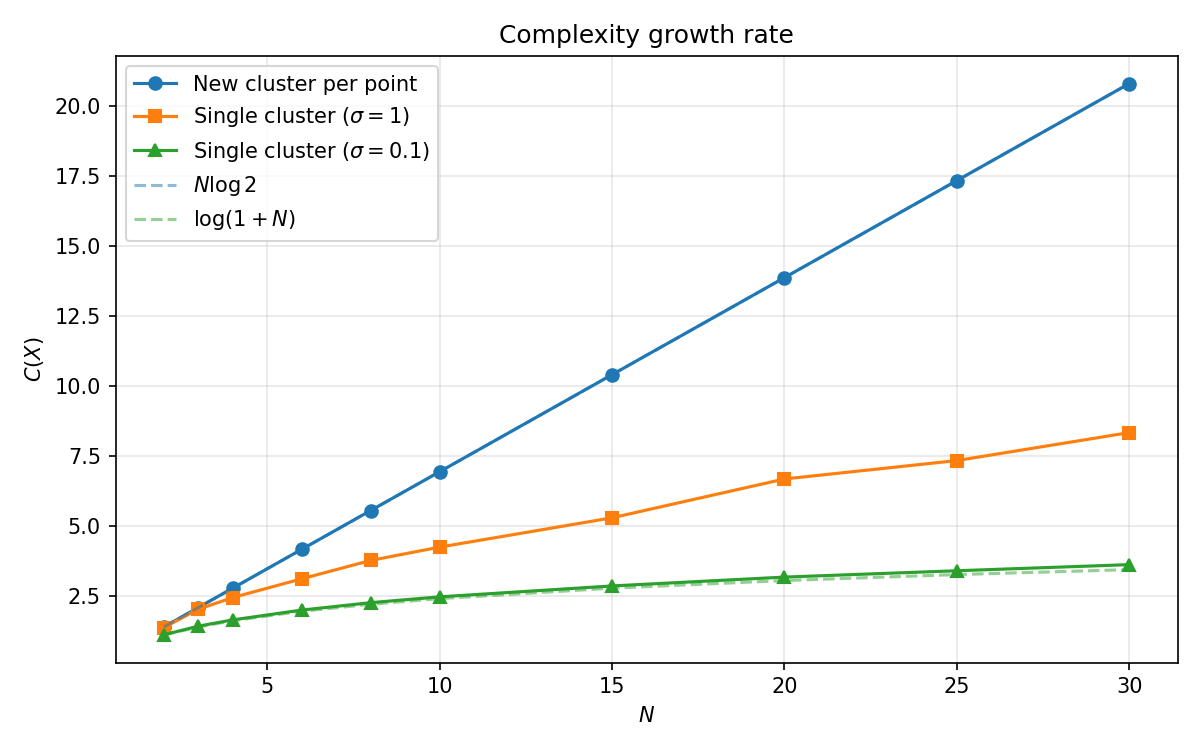
\includegraphics[width=0.75\linewidth]{growth_rate.png}
    \caption{Рост меры сложности $\mu_D(X)$ с объёмом выборки $N$ для выборок
    разной структуры. Синяя кривая: каждый объект образует новый независимый
    кластер, сложность растёт по верхней границе $N\log2$. Оранжевая и зелёная:
    все объекты из одного кластера с разбросом $\sigma=1$ и $\sigma=0{,}1$
    соответственно; для плотного кластера рост выходит на нижнюю границу
    $\log(1+N)$. Пунктиром показаны теоретические границы прироста.}
    \label{fig:growth}
\end{figure}
% TODO: численные наклоны и значения из exp3.

\subsection{Изображения MNIST}
\label{ssec:exp-mnist}
На предобученной диффузионной модели для изображений MNIST траектории вычисляются
численным интегрированием ОДУ вероятностного потока. Рис.~\ref{fig:mnist}
показывает, что мера согласована с семантическим разнообразием: выборка из
изображений одного класса (цифры~0) растёт с объёмом медленнее, чем выборка из
изображений разных классов. Отдельно проверяется выборка-орбита: набор из малых
сдвигов и поворотов одного изображения при большом числе объектов остаётся
низкосложным.
\begin{figure}[ht]
    \centering
    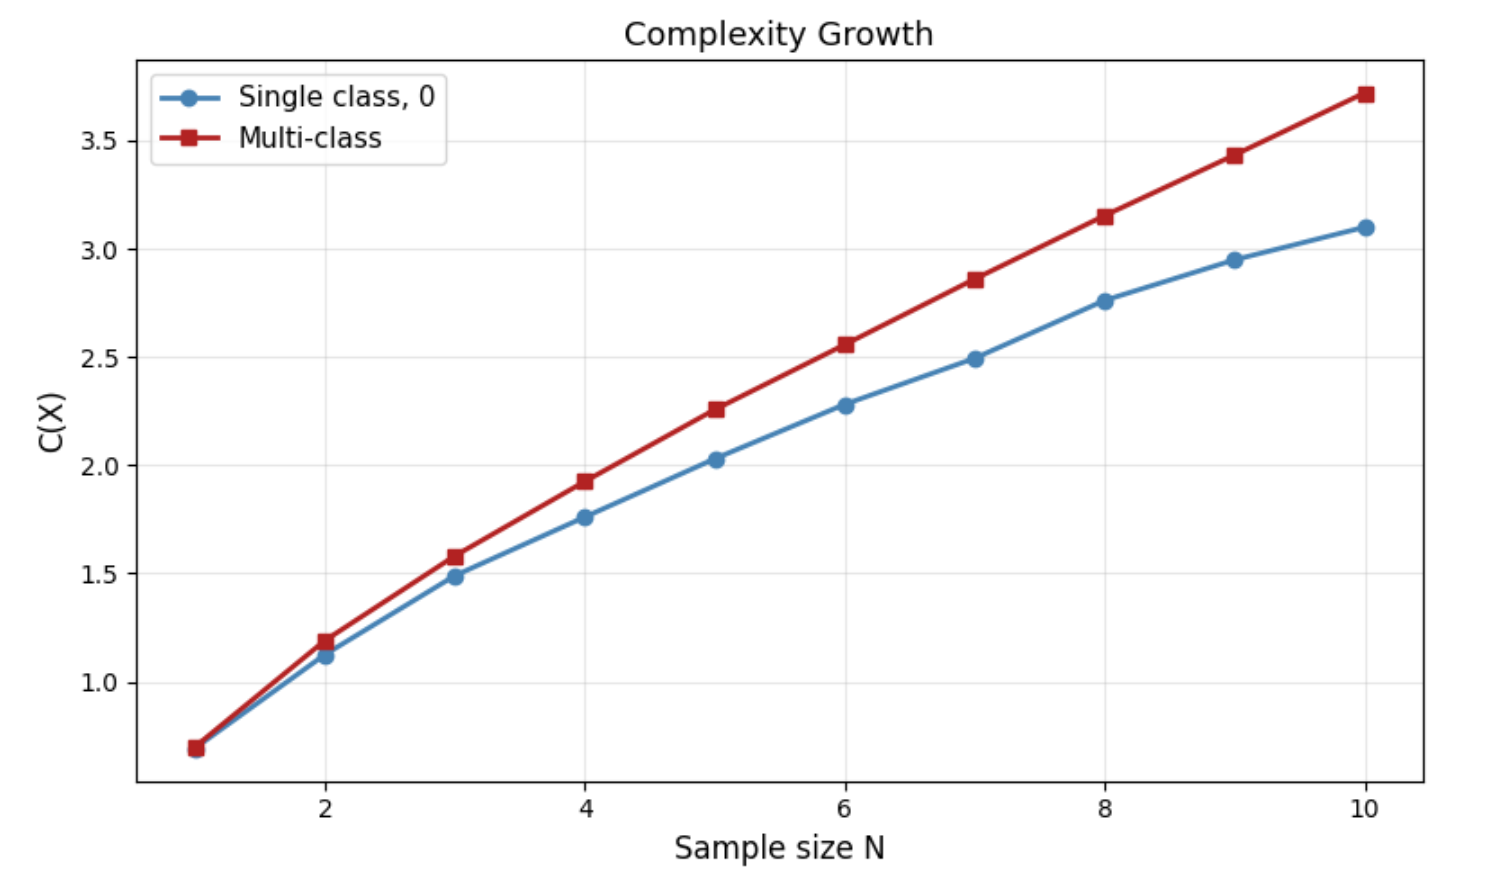
\includegraphics[width=0.75\linewidth]{Mnist_picture.png}
    \caption{Рост меры сложности $\mu_D(X)$ с объёмом выборки $N$ на изображениях
    MNIST. Выборка из изображений одного класса (цифра~0) имеет меньшую сложность,
    чем выборка из изображений разных классов.}
    \label{fig:mnist}
\end{figure}
% TODO: график зависимости mu_D от магнитуды преобразования (орбита) из exp4 (отдельной фигурой).

% ==========================================================================
\section{Заключение}
\label{sec:conclusion}
% ==========================================================================

В работе предложена и обоснована мера сложности обучающей выборки, учитывающая
семантическую геометрию данных, которая извлекается из предобученной диффузионной
модели. Поставленные задачи решены.

Формализовано понятие выборки, упорядоченной и допускающей повторы, и описаны
требования к мере сложности: инвариантность к перестановкам, субаддитивность и
монотонность. Показано, что для выборок с повторами монотонность не вытекает из
субаддитивности и является самостоятельным требованием.

Доказана теорема о достаточном условии корректности: для всякого положительно
полуопределённого ядра с единичной диагональю мера $\mu_D(X)=\log\det(I+K)$
обладает всеми тремя свойствами, причём прирост сложности при добавлении объекта
ограничен с обеих сторон точными границами
$\log\frac{N+2}{N+1}\le\Delta\le\log 2$. Установлены дополнительные свойства меры,
включая субмодулярность, а критерий Шёнберга описывает, какие ядра порождают
корректную меру.

Предложена реализация меры через траекторное вложение диффузионной модели. Каждому
объекту сопоставляется траектория ОДУ вероятностного потока, расстояние между
траекториями $D$ является метрикой при $p\in(0,2]$, а порождаемое ядро
$e^{-\lambda D^\beta}$ положительно полуопределено. Доказана липшицева устойчивость
меры к возмущению скор-функции. Вычислительные эксперименты показали, что мера
растёт вместе с семантическим разнообразием данных на синтетических наборах и на
изображениях MNIST.

Практическая значимость состоит в том, что мера не требует разметки данных и
снабжена доказанными гарантиями корректности. Она применима к оценке разнообразия
наборов данных, к отбору обучающих подвыборок и к сравнению выборок одного объёма,
но разного содержания. По форме мера принадлежит семейству спектральных мер
разнообразия и совпадает с информационным выигрышем гауссовского процесса. В
настоящей работе этот функционал обоснован как мера сложности выборки, снабжён
точными границами прироста и реализован через траектории диффузионной модели.

\textbf{План дальнейших исследований.}
\begin{itemize}
    \item \emph{Асимптотика меры.} Скорость роста $\mu_D(X)$ при $N\to\infty$
          определяется скоростью убывания спектра ядерного интегрального оператора
          и, как следствие, внутренней размерностью носителя распределения;
          представляет интерес строгое описание этой связи и режимов с
          согласованным масштабом $\lambda=\lambda_N$.
    \item \emph{Обоснованный выбор полосы $\lambda$.} Переход от калибровки на
          эталонной выборке к адаптивному выбору масштаба непосредственно по
          данным.
    \item \emph{Масштабирование.} Применение к крупным предобученным диффузионным
          моделям и другим модальностям (текст, аудио), а также вычислительно
          эффективная аппроксимация $\log\det$ больших ядерных матриц (методы
          Нистрёма, случайные проекции).
    \item \emph{Связь с обобщением.} Установление границ, связывающих $\mu_D$ с
          эффективностью обучения и обобщающей способностью моделей.
\end{itemize}

\newpage
\appendix
% ==========================================================================
\section{Доказательства}
\label{app:proofs}
% ==========================================================================

\begin{proof}[Доказательство теоремы~\ref{thm:lp}]
Обозначим $D(x,y)^2=\int_T\|\varphi_x(t)-\varphi_y(t)\|^{p}\,w(t)\,\mathrm{d}t$.

\emph{Условная отрицательная определённость $D^2$.} При каждом $t$ функция
$(x,y)\mapsto\|\varphi_x(t)-\varphi_y(t)\|^{p}
=\big(\|\varphi_x(t)-\varphi_y(t)\|^{2}\big)^{p/2}$ условно отрицательно
определена: квадрат евклидовой нормы УОО (теорема~\ref{thm:cnd}(iii)), а показатель
$p/2\le1$ сохраняет УОО (теорема~\ref{thm:cnd}, часть о степенях). Интегрирование с
весом $w\ge0$ сохраняет УОО: при $\sum_i c_i=0$
\[
    \sum_{i,j} c_i c_j\,D(x_i,x_j)^2
    =\int_T\Big(\sum_{i,j}c_ic_j\|\varphi_{x_i}(t)-\varphi_{x_j}(t)\|^{p}\Big)w(t)\,\mathrm{d}t\le0,
\]
так как подынтегральная сумма неположительна при каждом $t$. Значит $D^2$ условно
отрицательно определена, симметрична и имеет нулевую диагональ.

\emph{Метричность $D$.} По теореме~\ref{thm:cnd}(iii), применённой к $D^2$,
существуют гильбертово пространство $\mathcal{H}$ и отображение
$\Psi:x\mapsto\Psi(x)\in\mathcal{H}$ с
$D(x,y)^2=\|\Psi(x)-\Psi(y)\|_{\mathcal{H}}^2$, то есть
$D(x,y)=\|\Psi(x)-\Psi(y)\|_{\mathcal{H}}$. Отсюда симметрия, неотрицательность и
неравенство треугольника. Наконец, $D(x,y)=0$ равносильно $\varphi_x=\varphi_y$
($w$-почти всюду), а в силу инъективности отображения $x\mapsto\varphi_x$ это
равносильно $x=y$. Значит $D$~--- метрика.

\emph{Положительная полуопределённость ядра.} Так как $D^2$ условно отрицательно
определена и $\beta/2\le1$, степень $D^{\beta}=(D^2)^{\beta/2}$ также условно
отрицательно определена (теорема~\ref{thm:cnd}, часть о степенях). По
теореме~\ref{thm:cnd}(ii) ядро $e^{-\lambda D^{\beta}}$ положительно полуопределено
при всех $\lambda>0$.
\end{proof}

\begin{proof}[Доказательство утверждения~\ref{prop:c3-independent}]
Рассмотрим меру $\mu_D(X) = f(|X|)$, зависящую только от объёма выборки, где
$f(0) = 0$, $f(1) = 2$ и $f(n) = 1$ при $n \ge 2$. Она удовлетворяет (C1), так
как зависит лишь от $|X|$, и (C2), так как $f(m+n) \le f(m) + f(n)$ для всех
$m, n \ge 0$. Однако $f(2) = 1 < 2 = f(1)$, таким образом добавление второго объекта уменьшает
сложность. Условие (C3) нарушено.
\end{proof}

\begin{proof}[Доказательство теоремы~\ref{thm:valid}]

\

Матрица $K=K(X)$ положительно полуопределена (определение~\ref{def:psd}), поэтому
$I+K\succ 0$ и $\mu_D$ определена и неотрицательна.

\textbf{(C1)} Перестановка $\pi$ объектов заменяет $K$ на $PKP^{\!\top}$ с
матрицей перестановки $P$, и
$\det(I+PKP^{\!\top})=\det\!\big(P(I+K)P^{\!\top}\big)=\det(I+K)$, так что $\mu_D$
не меняется.

\textbf{(C2)} Матрица
$M=I+K(X\cup Y)=\begin{psmallmatrix}A&B\\ B^{\!\top}&C\end{psmallmatrix}$ с
$A=I+K(X)\succ0$, $C=I+K(Y)\succ0$ положительно определена. По формуле дополнения
Шура $\det M=\det A\cdot\det\!\big(C-B^{\!\top}A^{-1}B\big)$. Так как
$B^{\!\top}A^{-1}B\succeq0$, то $0\prec C-B^{\!\top}A^{-1}B\preceq C$; определитель
монотонен на конусе положительно определённых матриц
($0\prec S\preceq C\Rightarrow\det S\le\det C$, по теореме Вейля о собственных
числах), поэтому $\det M\le\det A\cdot\det C$ (неравенство Фишера, см.\
\cite[\S7.8]{HornJohnson2013}). Логарифмируя, получаем
$\mu_D(X\cup Y)\le\mu_D(X)+\mu_D(Y)$.

\textbf{(C3)} Пусть $\mathbf{b}=\big(k(\mathbf{x},\mathbf{x}_i)\big)_{i=1}^N$.
С учётом $k(\mathbf{x},\mathbf{x})=1$
\[
    I+K\big(X\cup(\mathbf{x})\big)
    =\begin{psmallmatrix}I+K&\mathbf{b}\\ \mathbf{b}^{\!\top}&2\end{psmallmatrix},
\]
дополнение Шура к блоку $I+K$ равно $s=2-\mathbf{b}^{\!\top}(I+K)^{-1}\mathbf{b}$, и
\[
    \Delta:=\mu_D\big(X\cup(\mathbf{x})\big)-\mu_D(X)=\log s .
\]
\emph{Верхняя граница.} Так как $(I+K)^{-1}\succ0$, то
$\mathbf{b}^{\!\top}(I+K)^{-1}\mathbf{b}\ge0$, откуда $s\le2$ и $\Delta\le\log 2$.

\emph{Нижняя граница.} Матрица
$\begin{psmallmatrix}K&\mathbf{b}\\ \mathbf{b}^{\!\top}&1\end{psmallmatrix}
=K\big(X\cup(\mathbf{x})\big)\succeq0$, поэтому для всех $\mathbf{u}\in\mathbb{R}^N$,
$t\in\mathbb{R}$ выполнено
$\mathbf{u}^{\!\top}K\mathbf{u}+2t\,\mathbf{b}^{\!\top}\mathbf{u}+t^2\ge0$;
минимизация по $t$ даёт
$(\mathbf{b}^{\!\top}\mathbf{u})^2\le\mathbf{u}^{\!\top}K\mathbf{u}$ для всех
$\mathbf{u}$. Положим $\mathbf{v}=(I+K)^{-1}\mathbf{b}$. Тогда
\[
    q:=\mathbf{b}^{\!\top}(I+K)^{-1}\mathbf{b}
      =\mathbf{v}^{\!\top}(I+K)\mathbf{v}
      =\|\mathbf{v}\|^2+\mathbf{v}^{\!\top}K\mathbf{v},
\]
а из предыдущего неравенства при $\mathbf{u}=\mathbf{v}$ имеем
$q^2=(\mathbf{b}^{\!\top}\mathbf{v})^2\le\mathbf{v}^{\!\top}K\mathbf{v}
=q-\|\mathbf{v}\|^2$. Нормировка ядра, применённая к расширенной выборке
$X\cup(\mathbf{x})$, даёт $|b_i|\le1$ (определение~\ref{def:psd}), откуда
$\|\mathbf{b}\|^2\le N$; по неравенству Коши--Буняковского
$q=\mathbf{b}^{\!\top}\mathbf{v}\le\|\mathbf{b}\|\,\|\mathbf{v}\|
\le\sqrt{N}\,\|\mathbf{v}\|$, то есть $\|\mathbf{v}\|^2\ge q^2/N$. Подставляя,
получаем $q^2\le q-q^2/N$, откуда
\[
    q\le\frac{N}{N+1},
    \qquad
    \Delta=\log(2-q)\ge\log\Big(2-\frac{N}{N+1}\Big)=\log\frac{N+2}{N+1}>0.
\]
\end{proof}

\begin{proof}[Доказательство следствия~\ref{cor:submodular}]
Зафиксируем объект $\mathbf{x}$. Как в доказательстве теоремы~\ref{thm:valid},
пункт~(C3), прирост сложности при добавлении $\mathbf{x}$ к подвыборке $S$ равен
\[
    \Delta_S := \mu_D\big(S\cup(\mathbf{x})\big)-\mu_D(S)=\log s_S,
    \qquad
    s_S=2-\mathbf{b}_S^{\!\top}\big(I+K(S)\big)^{-1}\mathbf{b}_S,
\]
где $\mathbf{b}_S=\big(k(\mathbf{x},\mathbf{s})\big)_{\mathbf{s}\in S}$ и учтено
$k(\mathbf{x},\mathbf{x})=1$. Так как $\log$ монотонен, утверждение равносильно
неравенству $s_B\le s_A$ при $A\subseteq B$: достаточно показать, что величина
$s_S$ не возрастает при расширении подвыборки.

Матрица $K\big(B\cup(\mathbf{x})\big)$ положительно полуопределена, поэтому
допускает грам-разложение: найдутся векторы $\{\phi_{\mathbf{s}}\}_{\mathbf{s}\in B}$
и $\phi_{\mathbf{x}}$ в некотором евклидовом пространстве, для которых
$\langle\phi_{\mathbf{u}},\phi_{\mathbf{v}}\rangle=k(\mathbf{u},\mathbf{v})$
(это канонический признаковый отображатель воспроизводящего ядерного
гильбертова пространства, \cite{Aronszajn1950}); в частности
$\|\phi_{\mathbf{x}}\|^2=k(\mathbf{x},\mathbf{x})=1$. Введём на $\mathbb{R}^{B}$
функционал
\[
    F(\mathbf{w})=1+\|\mathbf{w}\|^2
      +\Big\|\phi_{\mathbf{x}}-\sum_{\mathbf{s}\in B}w_{\mathbf{s}}\,\phi_{\mathbf{s}}\Big\|^2 .
\]
Дополнение Шура $s_S$ обладает вариационным представлением
\[
    s_S=\min_{\mathbf{w}\in\mathbb{R}^{S}}
        \Big(2-2\,\mathbf{b}_S^{\!\top}\mathbf{w}
              +\mathbf{w}^{\!\top}\big(I+K(S)\big)\mathbf{w}\Big)
       =\min_{\operatorname{supp}\mathbf{w}\subseteq S}F(\mathbf{w}) ,
\]
где первый минимум достигается в $\mathbf{w}^\ast=\big(I+K(S)\big)^{-1}\mathbf{b}_S$,
а второе равенство получается подстановкой $k(\mathbf{x},\mathbf{x})=1$ и тождества
$\mathbf{w}^{\!\top}K(S)\mathbf{w}-2\,\mathbf{b}_S^{\!\top}\mathbf{w}
=\big\|\phi_{\mathbf{x}}-\sum_{\mathbf{s}\in S}w_{\mathbf{s}}\phi_{\mathbf{s}}\big\|^2-1$.

Пусть $A\subseteq B$. Минимум, задающий $s_A$, берётся по векторам с носителем в
$A$, а минимум для $s_B$~--- по всем $\mathbf{w}\in\mathbb{R}^{B}$, то есть по более
широкому множеству при том же $F$. Поэтому
\[
    s_B=\min_{\mathbf{w}\in\mathbb{R}^{B}}F(\mathbf{w})
    \;\le\;
    \min_{\operatorname{supp}\mathbf{w}\subseteq A}F(\mathbf{w})=s_A ,
\]
откуда $\Delta_B=\log s_B\le\log s_A=\Delta_A$.
\end{proof}

\begin{proof}[Доказательство утверждения~\ref{prop:lipschitz}]
\emph{Шаг 1: оценки траекторий.} Для двух начальных условий
$\mathbf{x},\mathbf{x}'$ разность траекторий
$\boldsymbol{\delta}(t)=\mathbf{z}_{\mathbf{x}}(t)-\mathbf{z}_{\mathbf{x}'}(t)$
в силу интегральной формы~\eqref{eq:pfode} удовлетворяет
$\|\boldsymbol{\delta}(t)\|\le\|\mathbf{x}-\mathbf{x}'\|
+CL\int_0^t\|\boldsymbol{\delta}(\tau)\|\,\mathrm{d}\tau$, откуда по
неравенству Гронуолла
$\|\boldsymbol{\delta}(t)\|\le e^{CLt}\|\mathbf{x}-\mathbf{x}'\|$. Так как
$\mu_w$~--- вероятностная мера, отсюда
$\|\Phi(\mathbf{x})-\Phi(\mathbf{x}')\|_{\mathcal{H}}^2
=\int_0^1\|\boldsymbol{\delta}(t)\|^2\,\mathrm{d}\mu_w(t)
\le e^{2CL}\|\mathbf{x}-\mathbf{x}'\|^2$, то есть~(i). Аналогично для двух
полей при общем начальном условии: разность
$\widehat{\boldsymbol{\delta}}(t)
=\mathbf{z}_{\mathbf{x}}(t)-\widehat{\mathbf{z}}_{\mathbf{x}}(t)$
удовлетворяет
\[
    \|\widehat{\boldsymbol{\delta}}(t)\|
    \le C\int_0^t\big(L\|\widehat{\boldsymbol{\delta}}(\tau)\|
      +\varepsilon\big)\,\mathrm{d}\tau
    \le C\varepsilon t
      +CL\int_0^t\|\widehat{\boldsymbol{\delta}}(\tau)\|\,\mathrm{d}\tau,
\]
и по неравенству Гронуолла
$\|\widehat{\boldsymbol{\delta}}(t)\|\le C\varepsilon t\,e^{CLt}
\le C\varepsilon e^{CL}$; значит
$\|\Phi(\mathbf{x})-\widehat{\Phi}(\mathbf{x})\|_{\mathcal{H}}
\le C\varepsilon e^{CL}$ для всех $\mathbf{x}$.

\emph{Шаг 2: от ядра к мере.} Для ППО-матриц $K,K'$ с единичной диагональю
\[
    \big|\log\det(I+K')-\log\det(I+K)\big|
    \le\sum_{i\ne j}\big|K'_{ij}-K_{ij}\big| .
\]
Действительно, отрезок $K_\tau=K+\tau\Delta$, $\Delta=K'-K$, $\tau\in[0,1]$,
лежит в выпуклом конусе ППО-матриц, поэтому $I+K_\tau\succeq I$ обратима,
функция $f(\tau)=\log\det(I+K_\tau)$ дифференцируема и
$f'(\tau)=\operatorname{tr}\big((I+K_\tau)^{-1}\Delta\big)
=\sum_{i,j}\big[(I+K_\tau)^{-1}\big]_{ji}\,\Delta_{ij}$. Каждый элемент
матрицы не превосходит её спектральной нормы, а
$\|(I+K_\tau)^{-1}\|\le1$ из $I+K_\tau\succeq I$; так как $\Delta_{ii}=0$,
получаем $|f'(\tau)|\le\sum_{i\ne j}|\Delta_{ij}|$, и остаётся применить
теорему Лагранжа.

\emph{Шаг 3: от расстояний к ядру.} Функция $u\mapsto e^{-\lambda u^2}$
липшицева на $[0,\infty)$ с константой
$\sup_{u\ge0}2\lambda u\,e^{-\lambda u^2}=\sqrt{2\lambda/e}$, а по обратному
неравенству треугольника в $\mathcal{H}$ изменение расстояния $D$ не
превосходит суммарного сдвига вложений его аргументов. При замене
$\mathbf{x}_k\mapsto\mathbf{x}_k'$ меняются лишь $2(N-1)$ внедиагональных
записей ядра, каждая~--- не более чем на
$\sqrt{2\lambda/e}\,e^{CL}\|\mathbf{x}_k-\mathbf{x}_k'\|$ по шагу~1, что
вместе с шагом~2 даёт~(ii). При замене поля каждое из $N(N-1)$ внедиагональных
расстояний меняется не более чем на $2C\varepsilon e^{CL}$ (сдвигаются
вложения обоих аргументов, шаг~1), диагональ ядра остаётся единичной, и
шаг~2 даёт~(iii).
\end{proof}

\newpage
\printbibliography

\end{document}
